\chapter{数值模拟}
我们采用计算机来求解模型.为了简化编程,我们主要采用MATLAB矩阵实验室进行有限差分法的数值计算.\par
\section{扩散方程的模拟}
我们考虑这样简单的扩散方程,
\begin{equation}
\begin{cases}
\dfrac{\partial u}{\partial t}=\dfrac{\partial^ u}{\partial x^2}+2 & 0<x<1,t>0, \\
u(0,t)=u(1,t)=0,& t>1, \\
u(x,0)=sin(\pi x)+x(1-x).
\end{cases}
\end{equation}
我们采用六点差分格式来解这个方程,下面为用MATLAB编写的计算程序.
 \begin{lstlisting}[caption=六点差分格式,language=Matlab]
function [e]=six(dx,dt,t)
    m=1/dx;
    n=t/dt;
    u1=zeros(1,m+1);
    x=[1:m-1]*dx;
    u1([2:m])= sin(pi*x)+x.*(1 - x);
    r=dt/dx/dx;r2=2+2*r;r3=2-2*r;
    for i=1:m-1
	a(i,i)=r2;if i>1
	a(i-1,i)=-r;
	a(i,i-1)=-r;
	end;
    end
    for i=1:m-1
	b(i,i)=r3;
	if i>1
	    b(i-1,i)=r;
	    b(i,i-1)=r;
	end
    end
    u=zeros(n+1,m+1);
    u(n+1,:)=u1;
    for k=1:n
	b=b*(u(n+2-k,2:m))'+0.04;
	u(n+1-k,2:m)=inv(a)*b;
    end
    ut=u(1,:);
    x1=[0,x,1];
    plot(x1,ut,'*')
\end{lstlisting}
\begin{figure}[h]
 \centering
 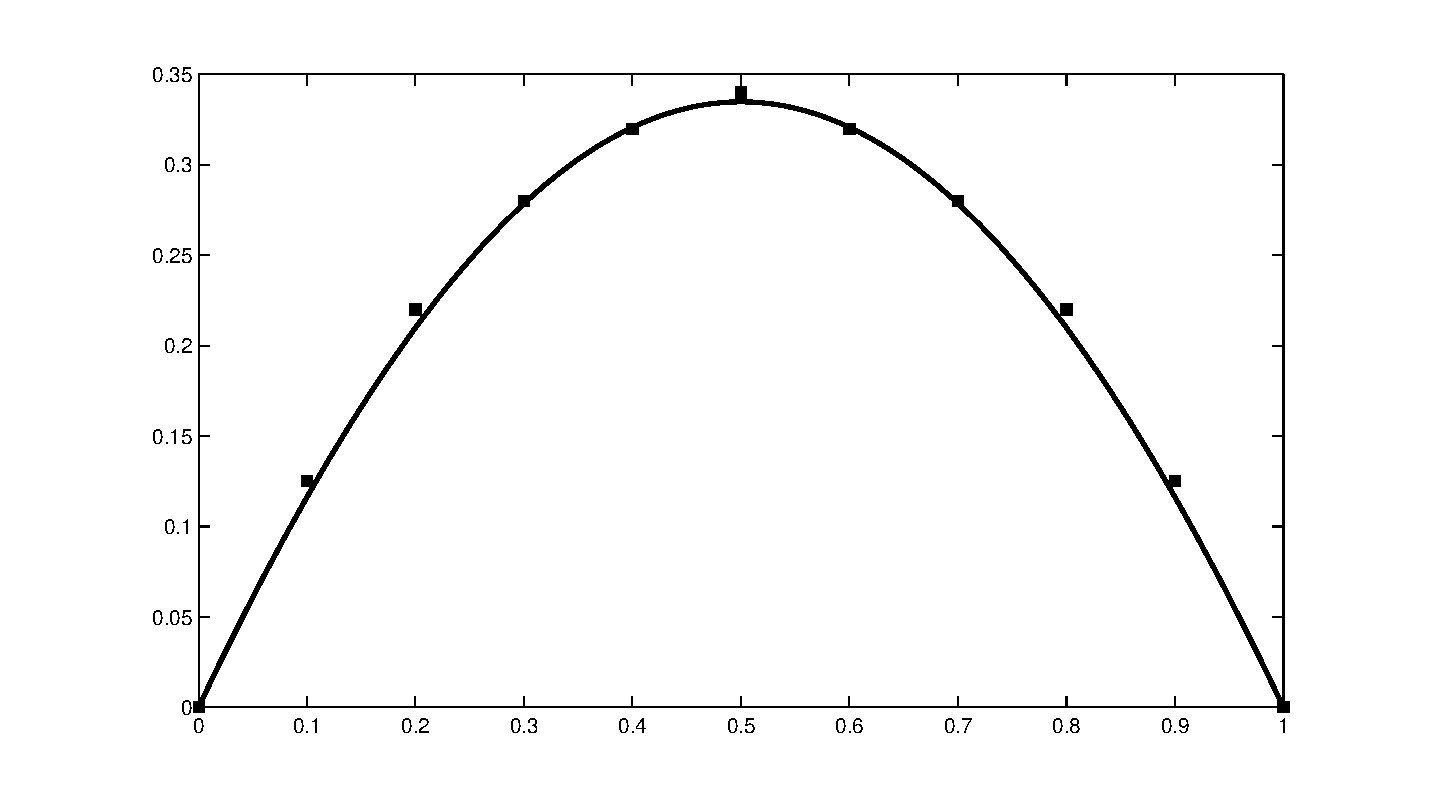
\includegraphics[scale=0.65]{./pic/6dcf.eps}
 \caption{扩散方程六点差分格式计算结果\label{fig:sm_ldcf}}
\end{figure}\par
仿真结果如图~\ref{fig:sm_ldcf}~所示,图中方块表示差分的数值结果,曲线表示解析结果.可以看到,虽然差分结果相对于解析解
是有误差的,但是误差不是很大.\newpage
\section{对流扩散方程的模拟}
